% ===============================================================
%  جلسه دوازدهم
% ===============================================================
\chapter{توابعی از یک متغیر تصادفی و تبدیل توزیع‌ها}

\section{یادآوری: تعریف مسئله و موارد ساده}

فرض کنید که متغیر تصادفی $X\sim f_X(x)$ و تابع دلخواه $g:\R\to\R$ داده شده باشند. متغیر تصادفی جدیدی به شکل $Y=g(X)$ را تشکیل می‌دهیم. هدف، به دست آوردن \textcolor{red!70!black}{تابع چگالی احتمال $f_Y(y)$} بر حسب $f_X(x)$ و $g(\cdot)$ است.

در جلسه قبل دو حالت ساده را دیدیم:
\begin{itemize}
\item \textbf{شیفت} $Y=X+b$: هر مقدار $Y$ از نمونه‌گیری از $X$ و سپس شیفت به اندازه $b$ حاصل می‌شود؛ پس
\[f_Y(y)=f_X(y-b).\]
\item \textbf{تبدیل خطی} $Y=aX+b$ با $a\ne0$:
\[
\begin{aligned}
f_Y(y)&=\lim_{h\to0}\frac{\Prob(y\le aX+b\le y+h)}{h}\\
&=\frac{1}{|a|}\lim_{h\to0}\frac{\Prob\big(\frac{y-b}{a}\le X\le\frac{y-b}{a}+\frac{h}{|a|}\big)}{h/|a|}=\frac{1}{|a|}f_X\Big(\frac{y-b}{a}\Big).
\end{aligned}
\]
\end{itemize}

\section{فرمول در حالت توابع $g$ یک‌به‌یک}

\begin{theorem}[تبدیل یک‌به‌یک]
فرض کنید که $g$ تابعی مشتق‌پذیر (با مشتق غیرصفر) و یک‌به‌یک باشد. در این صورت، فرض کنید به ازای مقدار معلوم $y$، مقدار یکتای $x^*$ را به صورت زیر تعریف کنیم:
\[
y=g(x^*)\qquad\text{or}\qquad x^*=g^{-1}(y).
\]
مشابه با روش گام به گام پیشین می‌توان نشان داد که:
\[
\boxed{\ f_Y(y)=\frac{1}{|g'(x^*)|}f_X(x^*)\ }
\]
\end{theorem}
(برای $g(x)=ax+b$ داریم $g'=a$ و $x^*=\frac{y-b}{a}$، که همان فرمول تبدیل خطی است.)

\section{فرمول کلی}

\begin{theorem}[تبدیل کلی]
فرض کنید که $g$ تابعی مشتق‌پذیر باشد. همچنین $x_1,x_2,\ldots$ را به صورت زیر تعریف می‌کنیم (همه ریشه‌های معادله $g(x)=y$):
\[
y=g(x_1)=g(x_2)=\cdots\qquad\text{or}\qquad\{x_1,x_2,\ldots\}=g^{-1}(y).
\]
در این صورت، می‌توان رابطه کلی را به صورت زیر نوشت:
\[
\boxed{\ f_Y(y)=\frac{1}{|g'(x_1)|}f_X(x_1)+\frac{1}{|g'(x_2)|}f_X(x_2)+\cdots\ }
\]
اگر معادله $g(x)=y$ هیچ ریشه‌ای نداشته باشد، $f_Y(y)=0$.
\end{theorem}

در صورتی که تابع $g$ در نقاطی مشتق‌پذیر نبود و یا مشتق آن صفر شد، معمولاً به صورت موردی باید تکلیف آن نقاط را مشخص نمود. (مثلاً اگر $g$ روی یک بازه با احتمال مثبت ثابت باشد، $Y$ در آن مقدار ثابت یک «ضربه» (دلتای دیراک) خواهد داشت.)

\section{بررسی و شهود ریاضیاتی}

\subsection{توجیه گرافیکی}
دلیل ظاهر شدن مشتق در رابطه پیشین چیست؟ یک تابع غیریکنوا مانند شکل زیر را در نظر بگیرید که بخش‌هایی صعودی (\lr{increasing}) و بخش‌هایی نزولی (\lr{decreasing}) دارد.

\begin{center}
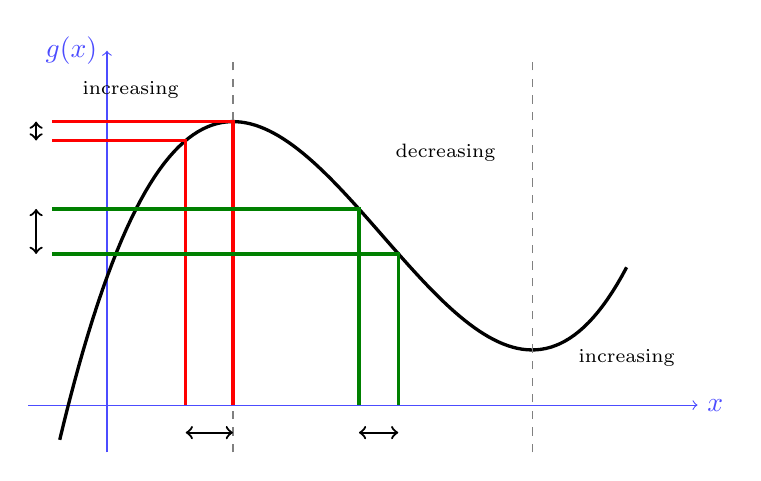
\begin{tikzpicture}[scale=1.0]
\draw[->,blue!70] (-1,0) -- (7.5,0) node[right]{$x$};
\draw[->,blue!70] (0,-0.6) -- (0,4.5) node[left]{$g(x)$};
\draw[very thick,domain=-0.6:6.6,samples=120] plot (\x,{0.3171*(\x*\x*\x/3-3.5*\x*\x+8.64*\x)+1.6247});
\draw[dashed,gray] (1.6,-0.6) -- (1.6,4.4);
\draw[dashed,gray] (5.4,-0.6) -- (5.4,4.4);
% big x-interval near the maximum -> small y-interval
\draw[red,very thick] (1.0,0) -- (1.0,3.36) -- (-0.7,3.36);
\draw[red,very thick] (1.6,0) -- (1.6,3.6) -- (-0.7,3.6);
\draw[<->,thick] (1.0,-0.35) -- (1.6,-0.35);
\draw[<->,thick] (-0.9,3.36) -- (-0.9,3.6);
% small x-interval in steep region -> big y-interval
\draw[green!50!black,very thick] (3.2,0) -- (3.2,2.49) -- (-0.7,2.49);
\draw[green!50!black,very thick] (3.7,0) -- (3.7,1.92) -- (-0.7,1.92);
\draw[<->,thick] (3.2,-0.35) -- (3.7,-0.35);
\draw[<->,thick] (-0.9,1.92) -- (-0.9,2.49);
\node[font=\scriptsize] at (0.3,4.0) {\lr{increasing}};
\node[font=\scriptsize] at (4.3,3.2) {\lr{decreasing}};
\node[font=\scriptsize] at (6.6,0.6) {\lr{increasing}};
\end{tikzpicture}
\end{center}

\begin{itemize}
\item \textbf{نزدیک بیشینه (شیب کم):} یک بازه \emph{بزرگ} از $x$ به یک بازه \emph{کوچک} از $y$ نگاشته می‌شود (خطوط قرمز در شکل). کل احتمال یک بازه بزرگ در یک بازه کوچک فشرده می‌شود؛ پس چگالی $Y$ آنجا \textbf{زیاد} است. چون $|g'|$ کوچک است، $\frac1{|g'|}$ بزرگ است.
\item \textbf{ناحیه پرشیب:} یک بازه \emph{کوچک} از $x$ به یک بازه \emph{بزرگ‌تر} از $y$ نگاشته می‌شود (خطوط سبز). احتمال کمی روی بازه بزرگی پخش می‌شود؛ پس چگالی $Y$ \textbf{کم} است. چون $|g'|$ بزرگ است، $\frac1{|g'|}$ کوچک است.
\item یک مقدار $y$ (خط افقی) ممکن است منحنی را در چند نقطه قطع کند؛ احتمال همه این شاخه‌ها با هم جمع می‌شود ــ از این‌رو در فرمول کلی جمع ظاهر شده است.
\end{itemize}
به زبان دقیق: برای $\dd y$ کوچک، $\Prob(y<Y\le y+\dd y)=\sum_i\Prob(X\in\text{بازه‌ای به طول }\frac{\dd y}{|g'(x_i)|}\text{ حول }x_i)\approx\sum_if_X(x_i)\frac{\dd y}{|g'(x_i)|}$.

\subsection{توجیه تحلیلی}
(برای سادگی) فرض کنید که $g$ تابعی اکیداً صعودی و لذا یک‌به‌یک باشد. در این صورت داریم:
\[
F_Y(y)=\Prob\big(g(X)\le y\big)=\Prob\big(X\le g^{-1}(y)\big)=F_X\big(g^{-1}(y)\big).
\]
مطابق قبل تعریف می‌کنیم $x^*=g^{-1}(y)$. با قاعده زنجیره‌ای:
\[
f_Y(y)=\frac{\partial}{\partial y}F_Y(y)=\frac{\partial g^{-1}(y)}{\partial y}\cdot\frac{\partial F_X\big(g^{-1}(y)\big)}{\partial g^{-1}(y)}=\frac{1}{g'(x^*)}f_X(x^*),
\]
که در آن از مشتق تابع معکوس $\frac{\dd g^{-1}(y)}{\dd y}=\frac{1}{g'(x^*)}$ استفاده شد. به دلیل فرض اکیداً صعودی بودن تابع، $g'>0$ و نیازی به قدرمطلق نیست.

اگر $g$ اکیداً نزولی باشد، $F_Y(y)=\Prob(X\ge g^{-1}(y))=1-F_X(g^{-1}(y))$ و مشتق آن $-\frac{f_X(x^*)}{g'(x^*)}=\frac{f_X(x^*)}{|g'(x^*)|}$ است (چون $g'<0$). قدرمطلق هر دو حالت را یکجا پوشش می‌دهد. برای $g$ غیریکنوا، دامنه را به بازه‌های یکنوا تقسیم کرده و سهم هر بازه را جمع می‌کنیم.

\section{مثال}

\begin{example}[مربع یک متغیر یکنواخت]
فرض کنید متغیر تصادفی $X$ توزیعی یکنواخت بین $-2$ تا $2$ دارد. متغیر تصادفی $Y$ را به صورت $Y=X^2$ تعریف می‌کنیم.
\begin{enumerate}
\item ساپورت $Y$ شامل چه مقادیری است؟
\item در کدام بخش‌های ساپورت، چگالی احتمال $Y$ خیلی زیاد می‌شود؟ در کدام بخش‌ها کم است؟
\item چگالی احتمال متغیر تصادفی $Y$، یعنی $f_Y(y)$ را به دست آورید.
\end{enumerate}
\begin{solution}
\textbf{۱. ساپورت:} چون $X\in[-2,2]$، داریم $Y=X^2\in[0,4]$.

\textbf{۲. شهود:} $g'(x)=2x$ نزدیک $x=0$ صفر است (شیب کم)؛ پس بازه‌ای از $x$ حول صفر به بازه بسیار کوچکی از $y$ نزدیک صفر فشرده می‌شود و چگالی $Y$ نزدیک $y=0$ \textbf{خیلی زیاد} (حتی بی‌نهایت) است. نزدیک $x=\pm2$ شیب زیاد است ($|g'|=4$)، پس چگالی $Y$ نزدیک $y=4$ \textbf{کم} است.

\textbf{۳. محاسبه:} $f_X(x)=\frac14$ برای $-2\le x\le2$. برای $0<y\le4$، معادله $x^2=y$ دو ریشه $x_{1,2}=\pm\sqrt y$ دارد و $|g'(x_{1,2})|=2\sqrt y$. طبق فرمول کلی:
\[
f_Y(y)=\frac{1}{2\sqrt y}\cdot\frac14+\frac{1}{2\sqrt y}\cdot\frac14=\frac{1}{4\sqrt y},\qquad0<y\le4,
\]
و $f_Y(y)=0$ در غیر این صورت.

\textbf{بررسی:} $\int_0^4\frac{\dd y}{4\sqrt y}=\frac14\big[2\sqrt y\big]_0^4=\frac14\times4=1$ \checkmark. همچنین $F_Y(y)=\Prob(|X|\le\sqrt y)=\frac{2\sqrt y}{4}=\frac{\sqrt y}{2}$ که مشتقش همان $\frac{1}{4\sqrt y}$ است.
\end{solution}
\end{example}

\begin{center}
\begin{tikzpicture}
\begin{axis}[width=6.5cm,height=4.8cm,axis lines=left,xmin=-2.5,xmax=2.5,ymin=0,ymax=0.5,title={\small $f_X(x)$},samples=2]
\addplot[blue,very thick] coordinates {(-2.5,0) (-2,0)};
\addplot[blue,very thick] coordinates {(-2,0.25) (2,0.25)};
\addplot[blue,very thick] coordinates {(2,0) (2.5,0)};
\end{axis}
\end{tikzpicture}
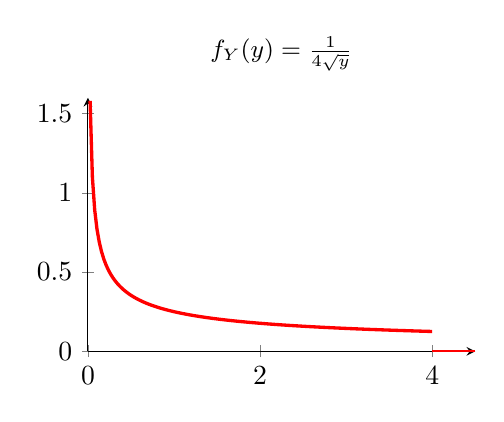
\begin{tikzpicture}
\begin{axis}[width=6.5cm,height=4.8cm,axis lines=left,xmin=0,xmax=4.5,ymin=0,ymax=1.6,title={\small $f_Y(y)=\frac{1}{4\sqrt y}$},samples=150]
\addplot[red,very thick,domain=0.025:4] {1/(4*sqrt(x))};
\addplot[red,very thick] coordinates {(4,0) (4.5,0)};
\end{axis}
\end{tikzpicture}
\end{center}

\begin{note}
\notetitle دقت کنید که $f_Y(y)\to\infty$ وقتی $y\to0^+$، ولی مساحت زیر آن متناهی (برابر ۱) است ــ نمونه دیگری از اینکه \lr{PDF} می‌تواند از ۱ بزرگ‌تر شود.
\end{note}

\section[تبدیل توزیع‌های مختلف به یکدیگر]{تبدیل توزیع‌های مختلف به یکدیگر {\large\lr{(Transforming Distributions)}}}

\subsection{تبدیل توزیع‌ها به توزیع یکنواخت}
\begin{theorem}[تبدیل انتگرال احتمال]
برای متغیر تصادفی (پیوسته) $X$ با توزیع انباشته دلخواه $F_X$، می‌توان مشاهده نمود که توزیع $Y=F_X(X)$ به صورت زیر محاسبه خواهد شد:
\[
f_Y(y)=\frac{f_X\big(F_X^{-1}(y)\big)}{F_X'\big(F_X^{-1}(y)\big)}=\ind(0\le y\le1).
\]
لذا $Y$ یک \textcolor{blue!60!black}{توزیع یکنواخت} بین صفر و یک خواهد داشت.
\end{theorem}
\begin{proof}
$g=F_X$ اکیداً صعودی است (روی تکیه‌گاه) و $g'=F_X'=f_X$. با فرمول تبدیل یک‌به‌یک و $x^*=F_X^{-1}(y)$: $f_Y(y)=\frac{f_X(x^*)}{f_X(x^*)}=1$ برای $y\in[0,1]$ (برد $F_X$). روش دوم با \lr{CDF}: $\Prob(Y\le y)=\Prob(F_X(X)\le y)=\Prob(X\le F_X^{-1}(y))=F_X(F_X^{-1}(y))=y$.
\end{proof}

\subsection{تبدیل توزیع یکنواخت به سایر توزیع‌ها}
\begin{theorem}[روش تبدیل معکوس]
فرض کنید که $f_Z,F_Z$ به ترتیب توابع چگالی و توزیع انباشته یک متغیر تصادفی فرضی مانند $Z$ باشند (دقت کنید که $f_Z$ و $F_Z$ توابعی معلوم و غیرتصادفی هستند). برای متغیر تصادفی $Y$ با توزیع یکنواخت $\mathcal U(0,1)$، می‌توان مشاهده نمود که توزیع متغیر تصادفی $F_Z^{-1}(Y)$ با متغیر تصادفی فرضی $Z$ یکسان خواهد بود.
\end{theorem}
\begin{proof}
$\Prob\big(F_Z^{-1}(Y)\le z\big)=\Prob\big(Y\le F_Z(z)\big)=F_Z(z)$، زیرا برای $Y$ یکنواخت $\Prob(Y\le u)=u$. پس \lr{CDF} متغیر $F_Z^{-1}(Y)$ دقیقاً $F_Z$ است.
\end{proof}

\begin{center}
\begin{tikzpicture}[>=Stealth,box/.style={draw,thick,rounded corners,minimum width=2.6cm,minimum height=1.1cm,align=center}]
\node[box,fill=blue!8] (X) at (0,0) {$X\sim F_X$\\ \small(هر توزیع)};
\node[box,fill=green!10] (U) at (5.6,0) {$U\sim\mathcal U(0,1)$};
\node[box,fill=red!8] (Z) at (11.2,0) {$Z\sim F_Z$\\ \small(توزیع دلخواه)};
\draw[->,very thick] (X) -- node[above]{$U=F_X(X)$} (U);
\draw[->,very thick] (U) -- node[above]{$Z=F_Z^{-1}(U)$} (Z);
\end{tikzpicture}
\end{center}
یعنی توزیع یکنواخت مانند یک «زبان مشترک» است: با ترکیب دو مرحله، هر توزیع پیوسته را می‌توان به هر توزیع دیگری تبدیل کرد: $Z=F_Z^{-1}(F_X(X))$.

\section{چگونگی تولید اعداد تصادفی}

کامپیوترها معمولاً تنها یک مولد \textbf{شبه‌تصادفی} از اعداد یکنواخت در $[0,1)$ دارند (مثلاً بر پایه «مولد هم‌نهشتی خطی» $s_{k+1}=(a\,s_k+c)\bmod m$ و $u_k=s_k/m$، یا الگوریتم‌های پیشرفته‌تری مانند \lr{Mersenne Twister}). سؤال: چگونه از این اعداد یکنواخت، نمونه‌هایی از توزیع‌های دیگر (نمایی، گاوسی، \ldots) تولید کنیم؟ پاسخ همان روش تبدیل معکوس است:

\begin{summarybox}[الگوریتم نمونه‌برداری با تبدیل معکوس \lr{(Inverse Transform Sampling)}]
\begin{enumerate}
\item یک عدد $u$ از $\mathcal U(0,1)$ تولید کنید.
\item $z=F_Z^{-1}(u)$ را خروجی دهید.
\end{enumerate}
\end{summarybox}

\begin{example}[تولید نمونه نمایی]
برای $Z\sim\mathrm{Exp}(\lambda)$ داریم $F_Z(z)=1-e^{-\lambda z}$. با حل $u=1-e^{-\lambda z}$:
\[
z=F_Z^{-1}(u)=-\frac{1}{\lambda}\ln(1-u).
\]
چون $1-U$ نیز یکنواخت است، می‌توان از $z=-\frac1\lambda\ln u$ هم استفاده کرد. مثلاً با $\lambda=2$ و $u=0.3$: $z=-\frac12\ln0.7\approx0.178$.
\end{example}

\begin{example}[تولید نمونه گسسته]
برای متغیر گسسته (مثلاً تاس)، تبدیل معکوس یعنی: $[0,1)$ را به بازه‌هایی با طول $p_1,p_2,\ldots$ تقسیم کنید و اگر $u$ در بازه $i$ام افتاد، مقدار $x_i$ را برگردانید. برای تاس سالم: $x=\lfloor6u\rfloor+1$.
\end{example}

\begin{note}
\notetitle برای گاوسی، $F^{-1}$ شکل بسته ندارد؛ در عمل از روش‌های دیگری مانند \textbf{تبدیل باکس--مولر} استفاده می‌شود: اگر $U_1,U_2$ یکنواخت و مستقل باشند، $Z=\sqrt{-2\ln U_1}\cos(2\pi U_2)$ گاوسی استاندارد است (این نتیجه از تبدیل دو متغیره به دست می‌آید که در جلسات بعد می‌بینیم).
\end{note}

\section{تمرین‌های تکمیلی}

\begin{exercise}
اگر $X\sim\mathcal U(0,1)$، چگالی $Y=-\ln X$ را بیابید.
\end{exercise}
\begin{solution}
$g(x)=-\ln x$ روی $(0,1)$ اکیداً نزولی است و برد آن $(0,\infty)$. $x^*=e^{-y}$ و $|g'(x^*)|=\frac{1}{x^*}=e^{y}$. پس $f_Y(y)=\frac{1}{e^y}\cdot1=e^{-y}$ برای $y>0$؛ یعنی $Y\sim\mathrm{Exp}(1)$ (همان نتیجه روش تبدیل معکوس).
\end{solution}

\begin{exercise}
اگر $X\sim\mathcal N(0,1)$، چگالی $Y=e^X$ را بیابید (توزیع لاگ‌نرمال).
\end{exercise}
\begin{solution}
$x^*=\ln y$ و $g'(x^*)=e^{x^*}=y$. پس برای $y>0$:
$f_Y(y)=\frac{1}{y}\cdot\frac{1}{\sqrt{2\pi}}e^{-(\ln y)^2/2}$ ــ همان لاگ‌نرمال جلسه هفتم با $\mu=0,\sigma=1$.
\end{solution}

\begin{exercise}
اگر $X\sim\mathcal U(0,\pi)$، چگالی $Y=\sin X$ را بیابید.
\end{exercise}
\begin{solution}
برد: $Y\in[0,1]$. برای $0<y<1$ دو ریشه دارد: $x_1=\arcsin y$ و $x_2=\pi-\arcsin y$؛ در هر دو $|g'|=|\cos x|=\sqrt{1-y^2}$. پس
$f_Y(y)=2\cdot\frac{1}{\pi}\cdot\frac{1}{\sqrt{1-y^2}}=\frac{2}{\pi\sqrt{1-y^2}}$، $0<y<1$. (بررسی: $\int_0^1\frac{2}{\pi\sqrt{1-y^2}}\dd y=\frac2\pi\cdot\frac\pi2=1$.)
\end{solution}

\begin{exercise}
یک الگوریتم برای تولید نمونه از توزیعی با چگالی $f(z)=2z$ روی $[0,1]$ بنویسید.
\end{exercise}
\begin{solution}
$F(z)=z^2$، پس $F^{-1}(u)=\sqrt u$. الگوریتم: $u\sim\mathcal U(0,1)$ تولید کن و $z=\sqrt u$ را برگردان. (معادلاً $\max(U_1,U_2)$ برای دو یکنواخت مستقل نیز همین توزیع را دارد، چون $\Prob(\max\le z)=z^2$.)
\end{solution}
